% Pengaturan ukuran teks dan bentuk halaman dua sisi
\documentclass[12pt]{book}

% Pengaturan ukuran halaman dan margin
\usepackage[a4paper,top=30mm,left=30mm,right=20mm,bottom=25mm]{geometry}

% Pengaturan ukuran spasi
\usepackage[singlespacing]{setspace}

% Pengaturan caption untuk tabel
\usepackage{caption}

% Judul dokumen
\title{Proposal Tugas Akhir ITS}
\author{Fajri, Dimas Aditya Maulana}

% Pengaturan detail pada file PDF
\usepackage[pdfauthor={\@author},bookmarksnumbered,pdfborder={0 0 0}]{hyperref}


% Pengaturan ukuran indentasi
\setlength{\parindent}{2em}

% Package lainnya
\usepackage{changepage}
\usepackage{etoolbox} % Mengubah fungsi default

% Pengaturan jenis karakter
\usepackage[utf8]{inputenc}

\usepackage[style=apa, backend=biber]{biblatex}
\usepackage{enumitem} % Pembuatan list
\usepackage{lipsum} % Pembuatan template kalimat
\usepackage{graphicx} % Input gambar
\usepackage{longtable} % Pembuatan tabel
\usepackage[table,xcdraw]{xcolor} % Pewarnaan tabel
\usepackage{eso-pic} % Untuk menggunakan background image di halaman
\usepackage{txfonts} % Font times
\usepackage{changepage} % Pembuatan teks kolom
\usepackage{multicol} % Pembuatan kolom ganda
\usepackage{multirow} % Pembuatan baris ganda
\usepackage{tabularx} % Untuk mengatur kolom, seperti grid pada CSS
\usepackage{wrapfig}

% Pengaturan format daftar isi, daftar gambar, dan daftar tabel
\usepackage[titles]{tocloft}
\setlength{\cftsecindent}{2em}
\setlength{\cftsubsecindent}{2em}
\setlength{\cftbeforechapskip}{1.5ex}
\setlength{\cftbeforesecskip}{1.5ex}
\setlength{\cftbeforetoctitleskip}{0cm}
\setlength{\cftbeforeloftitleskip}{0cm}
\setlength{\cftbeforelottitleskip}{0cm}
\renewcommand{\cfttoctitlefont}{\hfill\Large\bfseries} % command untuk membuat heading bold dan besar
\renewcommand{\cftaftertoctitle}{\hfill}
\renewcommand{\cftloftitlefont}{\hfill\Large\bfseries}
\renewcommand{\cftafterloftitle}{\hfill}
\renewcommand{\cftlottitlefont}{\hfill\Large\bfseries}
\renewcommand{\cftafterlottitle}{\hfill}

% Definisi untuk "Hati ini sengaja dikosongkan"
\patchcmd{\cleardoublepage}{\hbox{}}{
  \thispagestyle{empty}
  \vspace*{\fill}
  \begin{center}\textit{[Halaman ini sengaja dikosongkan]}\end{center}
  \vfill}{}{}

  % Pengaturan penomoran halaman
\usepackage{fancyhdr}
\fancyhf{}
\renewcommand{\headrulewidth}{0pt}
\pagestyle{fancy}
\fancyfoot[C,CO]{\thepage}
\patchcmd{\chapter}{plain}{fancy}{}{}
\patchcmd{\chapter}{empty}{plain}{}{}

% Pengaturan format judul bab
\usepackage{titlesec}
\renewcommand{\thesection}{\thechapter.\arabic{section}}
\titleformat{\chapter}[hang]{\centering\bfseries\large}{BAB\ \arabic{chapter}\ }{0ex}{\vspace{0ex}\centering}
\titleformat*{\section}{\large\bfseries}
\titleformat*{\subsection}{\normalsize\bfseries}
\titlespacing{\chapter}{0ex}{0ex}{4ex}
\titlespacing{\section}{0ex}{1ex}{0ex}
\titlespacing{\subsection}{0ex}{0.5ex}{0ex}
\titlespacing{\subsubsection}{0ex}{0.5ex}{0ex}
\setcounter{secnumdepth}{3} % Untuk memberi penomoran pada \subsubsection

\counterwithin{figure}{chapter}
\counterwithin{table}{chapter}

% Mengganti figure dan table menjadi gambar dan tabel
\renewcommand{\figurename}{Gambar}
\renewcommand{\tablename}{Tabel}

% Tambahkan format tanda hubung yang benar di sini
\hyphenation{
  ro-ket
  me-ngem-bang-kan
  per-hi-tu-ngan
}

% Menambahkan resource daftar pustaka
\addbibresource{pustaka/pustaka.bib}

% Isi keseluruhan dokumen
\begin{document}
  % Nomor halaman pembuka dimulai dari sini
  \pagenumbering{roman}

  % Atur ulang penomoran halaman
  \setcounter{page}{1}

  % Sampul Bahasa Indonesia
  \newcommand\covercontents{sampul/konten-id.tex}
  \AddToShipoutPictureBG*{
  \AtPageLowerLeft{
    % Ubah nilai berikut jika posisi horizontal background tidak sesuai
    \hspace{-3.25mm}

    % Ubah nilai berikut jika posisi vertikal background tidak sesuai
    \raisebox{0mm}{
      
\includegraphics[width=\paperwidth,height=\paperheight]{sampul/gambar/sampul-luar-tipis.png}
    }
  }
}

% Menyembunyikan nomor halaman
\thispagestyle{empty}

% Pengaturan margin untuk menyesuaikan konten sampul
\newgeometry{
  top=65mm,
  left=30mm,
  right=30mm,
  bottom=20mm
}

\begin{flushleft}

  % Pemilihan font sans serif
  \sffamily

  % Pemilihan font bold
  \fontseries{bx}
  \selectfont
  \begin{spacing}{1.5}
    \input{\covercontents}
  \end{spacing}

\end{flushleft}

\restoregeometry


  % Lembar pengesahan
  \begin{center}
  \large
  \textbf{LEMBAR PENGESAHAN}
\end{center}

% Menyembunyikan nomor halaman
\thispagestyle{empty}

\begin{center}
  \textbf{\tatitle{}}
\end{center}

\begingroup
% Pemilihan font ukuran small
\small

\begin{center}
  \textbf{TUGAS AKHIR}
  \\Diajukan untuk memenuhi salah satu syarat
  memperoleh gelar Sarjana Teknik pada \\
  Program Studi S-1 \studyprogram{} \\
  Departemen \department{} \\
  Fakultas \faculty{} \\
  Institut Teknologi Sepuluh Nopember
\end{center}

\begin{center}
  Oleh: \textbf{\name{}}
  \\NRP. \nrp{}
\end{center}

\begin{center}
  Disetujui oleh Tim Penguji Tugas Akhir:
\end{center}

\begingroup
% Menghilangkan padding
\setlength{\tabcolsep}{0pt}

\noindent
\begin{tabularx}{\textwidth}{X l}
  \advisor{}               & (Pembimbing I)                      \\
  NIP: \advisornip{}       &                                     \\
                           & ................................... \\
                           &                                     \\
                           &                                     \\
  \coadvisor{}             & (Pembimbing II)                     \\
  NIP: \coadvisornip{}     &                                     \\
                           & ................................... \\
                           &                                     \\
                           &                                     \\
  \examinerone{}.          & (Penguji I)                         \\
  NIP: \examineronenip{}   &                                     \\
                           & ................................... \\
                           &                                     \\
                           &                                     \\
  \examinertwo{}.          & (Penguji II)                        \\
  NIP: \examinertwonip{}   &                                     \\
                           & ................................... \\
                           &                                     \\
                           &                                     \\
  \examinerthree{}.        & (Penguji III)                       \\
  NIP: \examinerthreenip{} &                                     \\
                           & ................................... \\
\end{tabularx}
\endgroup

\begin{center}
  Mengetahui, \\
  Kepala Departemen \department{} \facultyshort{} - ITS\\

  \vspace{8ex}

  \underline{\headofdepartment{}.} \\
  NIP. \headofdepartmentnip{}
\end{center}

\begin{center}
  \textbf{\MakeUppercase{\place{}}\\\MONTH{}, \the\year{}}
\end{center}
\endgroup

  \cleardoublepage

  % Abstrak
  \chapter*{ABSTRAK}
\begin{center}
  \large
  \textbf{PREDIKSI JUMLAH KALORI YANG TERBAKAR SAAT BEROLAHRAGA DENGAN \emph{TREADMILL} BERBASIS KAMERA MENGGUNAKAN \emph{CONVOLUTIONAL NEURAL NETWORK}}
\end{center}
\addcontentsline{toc}{chapter}{ABSTRAK}
% Menyembunyikan nomor halaman
\thispagestyle{empty}

\begin{flushleft}
  \setlength{\tabcolsep}{0pt}
  \bfseries
  \begin{tabular}{ll@{\hspace{6pt}}l}
    Nama Mahasiswa / NRP&:& Dimas Aditya Maulana Fajri / 07211940000012\\
    Departemen&:& Teknik Komputer FTEIC - ITS\\
    Dosen Pembimbing&:& 1. Arief Kurniawan, S.T, M.T.\\
    & & 2. Dr. Eko Mulyanto Yuniarno, S.T, M.T.\\
  \end{tabular}
  \vspace{4ex}
\end{flushleft}
\textbf{Abstrak}

% Isi Abstrak
Obesitas merupakan keadaan dimana terdapat penumpukan lemak pada tubuh seseorang yang menyebabkan berat badan berada pada nilai di atas normal. Ketidak seimbangan kalori yang dikonsumsi dan yang digunakan menyebabkan kelebihan berat badan. Salah satu aktivitas yang bisa mengurangi kelebihan berat badan adalah dengan olahraga yang memiliki kualitas aktivitas yang baik. Olahraga pada treadmill merupakan salah satu aktivitas yang dapat dilakukan dan melakukan pengukuran kalori yang terbakar. Namun perhitungan kalori pada treadmill masih belum akurat dan praktis. Penelitian ini membuat sistem yang dapat memprediksi kalori yang terbakar saat olahraga pada treadmill menggunakan citra video dengan kamera. Metode yang digunakan dengan melakukan akuisisi data citra yang kemudian dideteksi dan estimasi pose untuk postur tubuh. Ekstrak hasil deteksi dilanjutkan untuk klasifikasi menggunakan CNN. Hasil deteksi berupa banyak langkah dan waktu untuk dilakukan prediksi kalori. Prediksi menggunakan regresi linear dengan variabel dependen jumlah kalori yang terbakar. Hasil akhir yang diharapkan dapat memprediksi jumlah kalori yang terbakar dari citra video.

\vspace{2ex}
\noindent
\textbf{Kata Kunci: \emph{Obesitas, Kalori, Prediksi, Citra}}
  \cleardoublepage

  \chapter*{ABSTRACT}
\begin{center}
  \large
  \textbf{PREDICTION OF CALORIES BURNED WHEN EXERCISING ON A \emph{TREADMILL} WITH CAMERA-BASED USING A \emph{CONVOLUTIONAL NEURAL NETWORK}}
\end{center}
% Menyembunyikan nomor halaman
\thispagestyle{empty}

\begin{flushleft}
  \setlength{\tabcolsep}{0pt}
  \bfseries
  \begin{tabular}{lc@{\hspace{6pt}}l}
  Student Name / NRP&: &Dimas Aditya Maulana Fajri / 07211940000012\\
  Department&: &Computer Engineering ELECTICS - ITS\\
  Advisor&: &1. Arief Kurniawan, S.T, M.T.\\
  & & 2. Dr. Eko Mulyanto Yuniarno, S.T, M.T.\\
  \end{tabular}
  \vspace{4ex}
\end{flushleft}
\textbf{Abstract}

% Isi Abstrak
Obesity is a condition where there is accumulation of fat in a person's body which causes the body weight to be above normal. Imbalance of calories consumed and used causes excess weight. One of the activities that can reduce excess weight is exercise that has good quality activities. Exercising on a treadmill is one of the activities that can be carried out and measures the calories burned. However, calculating calories on a treadmill is still not accurate and practical. This research creates a system that can predict calories burned while exercising on a treadmill using video images with a camera. The method used is by acquiring image data which is then detected and estimated for poses for body postures. Extract detection results are continued for classification using CNN. The results of the detection are in the form of many steps and time for calorie prediction. Prediction using linear regression with the dependent variable the number of calories burned. The final result is expected to be able to predict the number of calories burned from the video image.

\vspace{2ex}
\noindent
\textbf{Keywords: \emph{Obesity, Calories, Prediction, Image}}
  \cleardoublepage

  \begin{spacing}{1.5}
    % Daftar isi
    \renewcommand*\contentsname{DAFTAR ISI}
    \addcontentsline{toc}{chapter}{\contentsname}
    \tableofcontents
    \cleardoublepage

    % Daftar gambar
    \renewcommand*\listfigurename{DAFTAR GAMBAR}
    \addcontentsline{toc}{chapter}{\listfigurename}
    \listoffigures
    \cleardoublepage

    % Daftar tabel
    \renewcommand*\listtablename{DAFTAR TABEL}
    \addcontentsline{toc}{chapter}{\listtablename}
    \listoftables
    \cleardoublepage
  \end{spacing}

  % Nomor halaman isi dimulai dari sini
  \pagenumbering{arabic}

  % Konten pendahuluan
  \chapter{PENDAHULUAN}

\section{Latar Belakang}

% Ubah paragraf-paragraf berikut sesuai dengan latar belakang dari tugas akhir
Obesitas merupakan keadaan dimana terdapat penumpukan lemak pada tubuh seseorang yang menyebabkan berat badan berada pada nilai di atas normal. Indikasi yang dapat digunakan untuk menilai jika seseorang menderita obesitas berdasarkan nilai \emph{body mass index} (BMI) yang lebih dari 30 kg/m2. Obesistas disebabkan oleh kalori yang dikonsumsi tidak seimbang dengan kalori yang digunakan oleh tubuh. Salah satu hal yang dapat digunakan untuk mencegah obesitas dan mengurangi kelebihan berat badan dengan melakukan olahraga.

Olahraga merupakan suatu bentuk aktivitas fisik dalam kegiatan jasmani yang dilakukan secara terstruktur dengan melibatkan pergerakan tubuh secara berulang-ulang. Aktvitas olahraga dilakukan dengan tujuan untuk memelihara kesehatan dan memperkuat otot-otot tubuh. Olahraga menjadi kegiatan yang sangat dekat dengan aktivitas manusia sebagai salah satu kebutuhan hidup dalam memberikan manfaat berupa kesehatan dan kebugaran tubuh. 

Aktivitas olahraga dinilai bermanfaat dan sesuai prosedur dengan melihat bagaimana kualitas aktivitas olahraga yang telah dilakukan. Kualitas aktivitas olahraga dapat diukur berdasarkan jumlah energi yang dikeluarkan selama melakukan aktivitas olahraga. Energi yang dikeluarkan akan membantu meningkatkan jumlah pembakaran kalori pada tubuh. Jumlah energi yang dikeluarkan selama melakukan aktivitas olahraga akan berbeda-beda tergantung dari jenis aktivitas, durasi dan beberapa faktor pada individu.

\section{Rumusan Masalah}

% Ubah paragraf berikut sesuai dengan rumusan masalah dari tugas akhir
Aktivitas yang dilakukan pada treadmill dengan perhitungan pembakaran kalori hanya dapat dilakukan pada beberapa jenis treadmill yang memiliki sistem perhitungannya. Treadmill dengan sistem yang kompleks memungkinkan memiliki harga jual yang lebih tinggi dari treadmill yang sederhana. Sistem yang digunakan hanya bisa digunakan pada treadmill saja tanpa bisa terhubung satu sama lain antar alat. Hal ini membuat pengumpulan data dari setiap aktivitas yang dilakukan tidak tercatat dengan baik. Oleh karena itu, diperlukan sistem prediksi jumlah kalori yang terbakar yang lebih praktis dan mudah digunakan untuk berolahraga pada treadmill. 

\section{Batasan Masalah atau Ruang Lingkup}

Adapun batasan masalah dalam memfokuskan permasalahan yang dirumuskan pada penelitian ini adalah:

\begin{enumerate}[nolistsep]

    \item Metode yang digunakan dalam melakukan proses deteksi pose tubuh menggunakan Python dengan library OpenCV yaitu MediaPipe.
  
    \item Deteksi yang digunakan pada MediaPipe berfokus pada deteksi pose tubuh.
  
    \item Aktivitas fisik yang dideteksi berfokus hanya pada kegiatan olahraga menggunakan Treadmill.
    
    \item Akuisisi data citra diambil menggunakan perangkat kamera.
    
    \item Hasil deteksi berupa nilai prediksi perhitungan kalori yang terbakar selama aktivitas fisik yang dilakukan.

    \item Faktor kemiringan digunakan pada level 0 atau sama pada setiap percobaan.
  
\end{enumerate}

\section{Tujuan}

% Ubah paragraf berikut sesuai dengan tujuan penelitian dari tugas akhir
Tujuan dari penelitian tugas akhir ini adalah membuat sistem prediksi jumlah kalori yang terbakar saat berolahraga pada treadmill dengan melakukan prediksi kalori menggunakan citra dari kamera.

\section{Manfaat}

% Ubah paragraf berikut sesuai dengan tujuan penelitian dari tugas akhir
Adapun manfaat yang didapat pada penelitian ini adalah dapat membuat sistem yang lebih praktis dalam menentukan prediksi pembakaran kalori yang bisa digunakan disegala jenis treadmill dan dapat menggunakan satu sistem untuk berbagai macam jenis treadill dalam melakukan prediksi pebakaran kalori dalam penurunan berat badan.


  \cleardoublepage

  % Konten tinjauan pustaka
  \chapter{TINJAUAN PUSTAKA}

% Ubah konten-konten berikut sesuai dengan isi dari tinjauan pustaka
\section{Hasil penelitian/perancangan terdahulu}

\subsection{\emph{Analysis and Design of Calories Burning Calculation in Jogging Using Thresholding Based Accelerometer Sensor }(Okmuyura et al., 2019)}
  
Finanta Okmuyura, Noverta Effendi, Witri Ramadhani, dan Adlian Jefiza melakukan penelitian ini dengan membuat analisis dan desain untuk dapat memonitor pembakaran kalori saat jogging. Pada penelitian ini, dalam memonitor pembakaran kalori menggunakan sensor akselerometer yang dapat menghitung berdasarkan dari tekanan dari beban yang diterima untuk menghasilkan nilai \emph{threshold} untuk dikalkukasikan nantinya. Perhitungan kalori yang terbakar pada penelitian ini dengan menggunakan nilai jumlah langkah kaki, waktu dan berat pengguna untuk memberikan informasi pembakaran kalori dalam jogging.
  
\subsection{Sistem Prediksi Kalori Terbakar Pada Pesepeda Menggunakan \emph{Feedforward Neural Network} (Utami \& Ichwan, 2017)}
  
Dina Budhi Utami dan Muhammad Ichwan melakukan penelitian mengenai sistem prediksi kalori yang terbakar pada pesepeda menggunakan \emph{Feedforward Neural Network}. Penelitian ini melakukan prediksi berdasarkan detak jantung dan kecepatan kayuh saat bersepeda. Model prediksi kalori yang digunakan adalah \emph{Feedforward Neural Network} dengan arsitektur jaringan saraf tiruan terdiri dari 3 lapis. Hasil keluaran dari jaringan saraf tiruan adalah nilai prediksi kalori menggunakan pengujian 10000 data latih dengan memiliki tingkat kesalahan adalah 7\%.

\subsection{\emph{Estimating Physical Activity Intensity and Energy Expenditure Using Computer Vision on Videos} (Saponaro et al.,  2019)}
  
Pada tahun 2019, Philip Saponaro bersama Haoran Wei, Gregory Dominick dan Chandra Kambhamettu melakukan penelitian ini. Penelitian yang dilakukan mengenai perkirakan intensitas aktivitas fisik dan pengeluaran energi dengan menggunakan sistem visi komputer. Nilai perkiraan aktivitas fisik dan pengeluaran energi menggunakan faktor usia, jenis kelamin, kecepatan dan isyarat aktivitas. Data nilai usia dan jenis kelamin didapatkan dengan jaringan \emph{Deep Expectation} dan nilai aktivitas diperoleh dari perkiraan sudut sendi dan kecepatan gerak. Hasil yang didapat dengan akurasi nilai perkiraan aktivitas fisik sebesar 89,5\% dan perbedaan rata-rata pengeluaran energi sebesar 1,96 kCal/min.


\section{Teori/Konsep Dasar}

\subsection{Kalori}

Kalori merupakan pengukuran untuk menyatakan jumlah energi dalam makanan. Ketika makan dan minum, kita memberi kalori (energi) pada tubuh. Tubuh akan memakai kalori untuk bahan bakar aktivitas yang dilakukan. Banyaknya aktivitas yang dilakukan, maka banyak pula kalori (energi) yang dibutuhkan. Jumlah kalori dalam makanan dapat ditulis dalam satuan ‘kkal’ (kilokalori). Kalori adalah kebutuhan yang sangat penting bagi semua orang untuk kelangsungan hidupnya. Kalori merupakan hal utama sebagai penyokong tubuh dalam melakukan berbagai aktivitas (Inmawati N. D., 2016). 

Kebutuhan kalori bisa dihitung berdasarkan gender, umur, tinggi dan berat badan, komposisi tubuh, aktivitas, serta kondisi fisik seseorang. Kebutuhan kalori laki-laki berbeda dengan perempuan meskipun rentang umurnya sama. Jika kegiatan yang dilakukan membutuhkan aktivitas fisik yang lebih berat, maka kebutuhan akan asupan kalori harian meningkat. Mengetahui kebutuhan energi per hari bisa membantu menjaga kesehatan karena hal tersebut dapat mempengaruhi keseimbangan energi harian seseorang. Semakin banyak jenis makanan yang memiliki kandungan rendah kalori, atau masyarakat sering menyebutnya sebagai \emph{low fat}. Banyak sekali masyarakat yang tidak terakomodasi dengan baik perhatiannya akan kalori tersebut.

Tidak ada cara akurat untuk menghitung kalori. Beberapa faktor seperti berat badan, intensitas aktifitas, kondisi tubuh dan metabolisme. Aktivitas fisik akan membakar energi dalam tubuh sehingga jika asupan kalori ke dalam tubuh berlebihan dan tidak diimbangi dengan aktivitas fisik yang seimbang akan menyebabkan tubuh mengalami kegemukan. Semakin tua usia seseorang, kurang aktif bergerak menyebabkan massa otot dalam tubuh cenderung menurun dan kehilangan otot menyebabkan perlambatan tingkat pembakaran kalori dalam tubuh. Semakin bertambah usia dan dengan asupan kalori yang tetap, tubuh semakin sulit untuk membakar kalori yang masuk sehingga terjadi penumpukan energi didalam tubuh dan berdampak pada obesitas (Widiantini et al., 2013).

\subsection{Regresi Linear}

Regresi linier merupakan satu cara prediksi yang menggunakan garis lurus untuk menggambarkan hubungan diantara dua variabel (atau lebih) (Kurniawan, 2008). Regresi linier merupakan salah satu metode statistika yang digunakan untuk membentuk model hubungan antara variabel terikat (dependen; respon; Y) dengan satu atau lebih variabel bebas (independen, prediktor, X).  Apabila banyaknya variabel bebas hanya ada satu, disebut sebagai regresi linier sederhana, sedangkan apabila terdapat lebih dari 1 variabel bebas, disebut sebagai regresi linier berganda. Analisis regresi merupakan metode statistika yang banyak digunakan dalam penelitian. Istilah regresi pertama kali diperkenalkan oleh Sir Francis Galton pada tahun 1986.  Secara umum, analisis regresi adalah kajian terhadap hubungan satu variabel yang disebut sebagai variabel yang diterangkan dengan satu atau dua variabel yang menerangkan (Syilfi \& Ispriyanti, 2012). Variabel yang diterangkan selanjutnya disebut sebagai variabel respon, sedangkan variabel yang menerangkan biasa disebut variabel bebas. 

Terdapat 3 kegunaan dalam penggunaan regresi liner, diantaranya yaitu untuk tujuan deskripsi dari fenomena data atau kasus yang sedang diteliti, untuk tujuan kontrol, serta untuk tujuan prediksi. Regresi mampu mendeskripsikan fenomena data melalui terbentuknya suatu model hubungan yang bersifatnya numerik. Regresi juga dapat digunakan untuk melakukan pengendalian (kontrol) terhadap suatu kasus atau hal-hal yang sedang diamati melalui penggunaan model regresi yang diperoleh. Selain itu, model regresi juga dapat dimanfaatkan untuk melakukan prediksi untuk variabel terikat. Namun yang perlu diingat, prediksi di dalam konsep regresi hanya boleh dilakukan di dalam rentang data dari variabel-variabel bebas yang digunakan untuk membentuk model regresi tersebut. Misal, suatu model regresi diperoleh dengan mempergunakan data variabel bebas yang memiliki rentang antara 5 s.d. 25, maka prediksi hanya boleh dilakukan bila suatu nilai yang digunakan sebagai input untuk variabel X berada di dalam rentang tersebut. Konsep ini disebut sebagai interpolasi (Sulardi et al., 2017).

Data untuk variabel independen X pada regresi linier bisa merupakan data pengamatan yang tidak ditetapkan sebelumnya oleh peneliti (\emph{obsevational data}) maupun data yang telah ditetapkan (dikontrol) oleh peneliti sebelumnya (\emph{experimental or fixed data}). Perbedaannya adalah bahwa dengan menggunakan \emph{fixed data}, informasi yang diperoleh lebih kuat dalam menjelaskan hubungan sebab akibat antara variabel X dan variabel Y. Sedangkan, pada \emph{observational data}, informasi yang diperoleh belum tentu merupakan hubungan sebab-akibat. Untuk \emph{fixed data}, peneliti sebelumnya telah memiliki beberapa nilai variabel X yang ingin diteliti. Sedangkan, pada \emph{observational data}, variabel X yang diamati bisa berapa saja, tergantung keadaan di lapangan. Biasanya, \emph{fixed data} diperoleh dari percobaan laboratorium, dan \emph{observational data} diperoleh dengan menggunakan kuesioner.

\subsection{Deteksi Gestur Tubuh}

Deteksi gestur tubuh atau yang dapat disebut \emph{body pose recognition} merupakan teknologi yang mampu membaca gerak pose tubuh kemudian menjadikan proses yang diinginkan oleh peneliti. Deteksi gestur ini merupakan topik dalam \emph{computer science} yang memiliki tujuan agar komputer dapat memahami gerakan manusia yang berasal dari postur tubuh.

\subsection{\emph{Deep Learning}}

\emph{Deep learning} adalah salah satu bidang \emph{machine learning} yang memanfaatkan banyak \emph{layer} pengolahan informasi nonlinier untuk melakukan ekstraksi fitur, pengenalan pola, dan klasifikasi (Deng dan Yu, 2014). Menurut Goodfellow, dkk. (2016), \emph{Deep learning} adalah sebuah pendekatan dalam penyelesaian masalah pada sistem pembelajaran komputer yang menggunakan konsep hierarki. Konsep hierarki membuat komputer mampu mempelajari konsep yang kompleks dengan menggabungkan dari konsep-konsep yang lebih sederhana. Jika digambarkan sebuah graf bagaimana konsep tersebut dibangun di atas konsep yang lain, graf ini akan dalam dengan banyak layer, hal tersebut menjadi alasan disebut sebagai \emph{Deep learning} (pembelajaran mendalam).

\emph{Deep learning} terdiri dari banyak lapisan (\emph{hidden layer}) dan membentuk tumpukan, lapisan tersebut adalah sebuah algoritma atau metode yang melakukan klasifikasi perintah yang diinput hingga menghasilkan \emph{output}. Metode \emph{deep learning} yang sedang berkembang salah satunya adalah \emph{Convolutional Neural Network}. Jaringan ini menggunakan masukan berupa gambar, kemudian akan melalui lapisan konvolusi dan diolah berdasarkan filter yang ditentukan, setiap lapisan ini menghasilkan pola dari beberapa bagian citra yang memudahkan proses klasifikasi (Danukusumo, 2017).

Metode \emph{Deep Learning} yang saat ini memiliki hasil paling signifikan dalam pengenalan citra adalah \emph{Convolutional Neural Network} (CNN) (Nugroho et al., 2020). Hal tersebut dikarenakan CNN berusaha meniru sistem pengenalan citra pada visual cortex manusia sehingga memiliki kemampuan mengolah informasi citra. Namun, CNN seperti metode \emph{Deep Learning} lainnya, memiliki kelemahan yaitu proses pelatihan model yang lama. Dengan perkembangan perangkat keras, hal tersebut dapat diatasi menggunakan teknologi \emph{General Purpose Graphical Processing Unit} (GPGPU). CNN dirancang khusus untuk pengenalan dan klasifikasi gambar. CNN memiliki beberapa lapisan (\emph{layer}) yang mengekstrak informasi dari gambar dan menentukan klasifikasi dari gambar berupa skor klasifikasi.


\subsection{\emph{Convolutional Neural Network}}

\emph{Convolutional Neural Network} (CNN) adalah salah satu jenis perhitungan \emph{neural network} yang sering digunakan pada pengolahan citra untuk mendeteksi dan mengenali objek pada sebuah \emph{image} (Mehindra, 2020). CNN berupa jaringan saraf yang dikhusukan untuk memproses data yang memiliki grid. CNN juga dapat diartikan sebagai kombinasi dari jaringan syaraf tiruan dan metode \emph{deep learning} (Fonda, 2020). CNN terdiri dari satu atau lebih lapisan konvolutional, seringnya dengan suatu lapisan \emph{dubsampling} yang diikuti oleh satu atau lebih lapisan yang terhubung penuh sebagai standar jaringan syaraf.

Arsitektur dari CNN juga terbagi menjadi 2 bagian besar yaitu \emph{Feature Extraction Layer} dan \emph{Fully-Connected Layer} (MLP). Sebuah CNN terdiri dari beberapa layer. Berdasarkan aristektur LeNet5, terdapat empat macam layer utama pada sebuah CNN yaitu \emph{Convolution Layer, Pooling Layer, Subsampling Layer,} dan \emph{Fully Connected Layer} (Eka Putra, 2016).

Pada CNN, data yang dipropagasikan oleh jaringan adalah data dua dimensi, sehingga operasi linear dan parameter bobot pada CNN berbeda. Pada CNN operasi linear menggunakan operasi konvolusi, sedangkan bobot tidak lagi satu dimensi saja, namun berbentuk empat dimensi yang merupakan kumpulan kernel konvolusi. Karena sifat proses konvolusi, maka CNN hanya dapat digunakan pada data yang memiliki struktur dua dimensi seperti citra dan suara.

Sebagai contoh adalah berupa citra dua dimensi. Nama konvolusi sendiri merupakan operasi aljabar linear yang mengkalikan matriks dari filter pada citra yang akan di proses. Proses ini disebut lapisan konvolusi dan merupakan salah satu jenis dari banyak lapisan bisa dimiliki dalam satu jaringan. Lapisan konvolusi merupakan lapisan utama yang paling penting untuk digunakan. Jenis lapisan lain yang biasa digunakan adalah \emph{Pooling Layer}, yakni lapisan yang digunakan untuk mengambil nilai maksimal atau nilai rata-rata dari bagian-bagian piksel pada citra. Setiap lapisan input yang dimasukkan memiliki volume yang berbeda da mewakili dengan kedalaman, tinggi dan lebar. Setiap besaran yang didapatkan tergantung dari hasil filtrasi dari lapisan sebelumnya dan juga banyak filter yang digunakan. Model jaringan seperti ini sudah terbukti sangat ampuh dalam menangani permasalahan klasifikasi citra. 


\subsection{Mediapipe}

Mediapipe adalah kerangka kerja yang terutama digunakan untuk menghasilkan audio atau video Dengan bantuan \emph{framework} MediaPipe, \emph{pipeline Machine Learning} dapat dibuat untuk instance model inferensi seperti TensorFlow, TFLite, dan juga untuk fungsi pemrosesan media, bahkan tidak memerlukan GPU untuk menjalankan eksperimen dengan MediaPipe, karena grafik dan CPU terintegrasi saat ini bekerja dengan baik untuk solusi ini. Logikanya, FPS jauh lebih rendah daripada penggunaan GPU, tampak pada gambar 2.2.

% Contoh input gambar dengan format *.jpg
\begin{figure} [ht] \centering
  % Nama dari file gambar yang diinputkan
  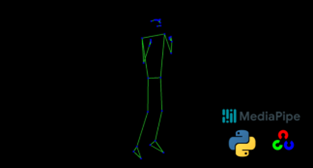
\includegraphics[scale=1]{gambar/mediapipe.png}
  % Keterangan gambar yang diinputkan
  \caption{Mediapipe untuk Pose Estimation}
  % Label referensi dari gambar yang diinputkan
  \label{fig:Mediapipe}
\end{figure}



  \cleardoublepage

  % Konten metodologi
  \chapter{METODOLOGI}

% Ubah konten-konten berikut sesuai dengan isi dari metodologi

\section{Metode yang digunakan}

% Contoh input gambar dengan format *.jpg
\begin{figure} [ht] \centering
  % Nama dari file gambar yang diinputkan
  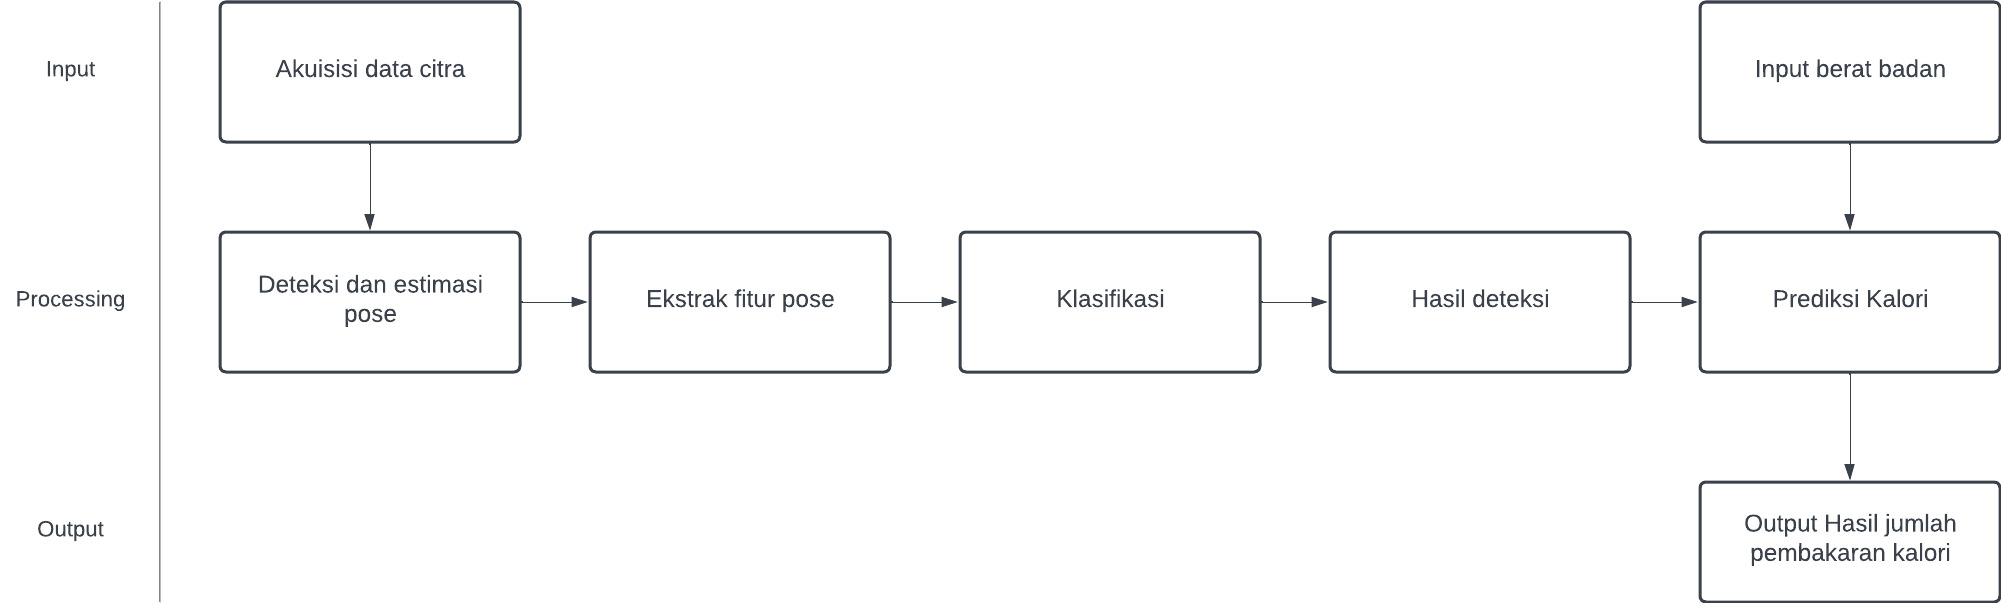
\includegraphics[scale=0.9]{gambar/blok diagram metodologi.jpeg}
  % Keterangan gambar yang diinputkan
  \caption{Blok Diagram Kerja Sistem}
  % Label referensi dari gambar yang diinputkan
  \label{fig:BlokDiagram}
\end{figure}

  \subsection{Akuisisi data citra}

  Pada tahap pertama yaitu akuisisi data citra, data diperoleh menggunakan kamera Webcam yang dimiliki oleh laptop atau kamera Webcam eksternal yang dihubungkan pada laptop ataupun komputer. Proses akuisisi data citra dilakukan dengan peraga melakukan aktivitas pada treadmill dengan ditampakkan secara jelas pada tampilan kamera Webcam. Setelah terdapat peraga dan tampak jelas pada tampilan maka data citra akan dilakukan pada tahap selanjutnya untuk dideteksi dan segmentasi pose seperti pada Gambar \ref{fig:AkuisisiData}.

  % Contoh input gambar dengan format *.jpg
  \begin{figure} [ht] \centering
    % Nama dari file gambar yang diinputkan
    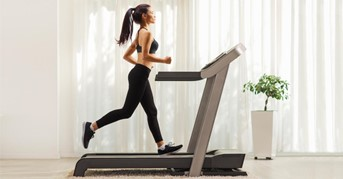
\includegraphics[scale=1.2]{gambar/akuisisi data.jpg}
    % Keterangan gambar yang diinputkan
    \caption{Posisi kamera untuk akuisisi data citra}
    % Label referensi dari gambar yang diinputkan
    \label{fig:AkuisisiData}
  \end{figure}
  
  \subsection{Deteksi dan estimasi pose}

  Deteksi dari hasil citra untuk dapat mengetahui bentuk postur tubuh manusia menggunakan Python dengan \emph{library} OpenCV yaitu MediaPipe. Metode yang digunakan pada MediaPipe menggunakan deteksi pose untuk mendeteksi postur tubuh. Segementasi dilakukan dengan cara peraga melakukan aktivitas jogging pada treadmill dengan menentukan pose melangkah seperti yang terdapat pada Gambar \ref{fig:DeteksiEstimasi}.

  % Contoh input gambar dengan format *.jpg
  \begin{figure} [ht] \centering
    % Nama dari file gambar yang diinputkan
    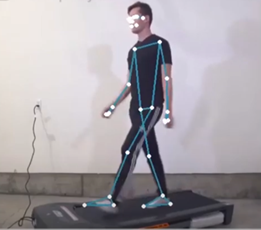
\includegraphics[scale=1.1]{gambar/deteksi estimasi.png}
    % Keterangan gambar yang diinputkan
    \caption{Deteksi dan estiasi pose dengan MediaPipe}
    % Label referensi dari gambar yang diinputkan
    \label{fig:DeteksiEstimasi}
  \end{figure}

  \subsection{Ekstrak fitur pose}

  Fitur dibuat berdasarkan segmentasi pose yang telah ditentukan dan dilakukan deteksi. Semua fitur dipersiapkan sebagai kombinasi dataset yang nantinya akan digunakan pada training. Setelah menentukan fitur yang akan diekstrak, dilakukan ekstrak fitur untuk mendapatkan setiap data yang dibutuhkan dengan setiap percobaan dari kombinasi segmentasi pose. Hasil yang didapat dari ekstrak fitur berupa data set yang nantinya akan dilakukan training untuk model yang diinginkan.

  \subsection{Klasifikasi}

  Fitur yang telah dilakukan ekstraksi maka kemudian dilakukan \emph{training} untuk memperoleh model deteksi. Model deteksi dari data set akan digunakan untuk melatih model dari sebuah algoritma pada \emph{Machine Learning}. Dalam melakukan klasifikasi menggunakan \emph{Convolutional Neural Networks} (CNN). Proses training ini bertujuan agar nantinya komputasi yang dilakukan dalam proses deteksi akan dapat diolah berdasarkan akuisisi data citra menjadi bentuk atau pola pemahaman yang diinginkan. Proses \emph{training} dilakukan dengan metode \emph{activity recognition} untuk dapat menklasifikasikan suatu aktivitas. Dengan begitu, dalam proses \emph{training} digunakan beberapa \emph{frame} dari fitur yang sudah diekstraksi untuk bisa diklasifikasikan dalam bentuk deteksi aktivitas. Klasifikasi dalam menentukan aktivitas yang digunakan pada penelitian ini adalah dapat mengetahui langkah dari seseorang yang berjalan atau berlari.

  \subsection{Hasil deteksi}

  Setelah dilakukan training dan klasifikasi, akan didapat model deteksi yang diinginkan. Bentuk hasil klasifikasi yang dibuat adalah mendeteksi pose aktivitas dengan dapat menghitung langkah dan waktu yang ditempuh. Nilai langkah dan waktu yang ditempuh akan digunakan dalam perhitungan selanjutnya.

  \begin{enumerate}[listparindent=2em]
    \item[\textbf{1.}] \textbf{Hasil deteksi langkah}
    
    Banyaknya jumlah langkah yang didapat saat hasil deteksi digunakan sebagai nilai variable pertama yang akan digunakan dalam penentuan perhitungan kalori. Langkah dideteksi dan dihitung seberapa banyak langkah yang dilakukan saat proses deteksi. Nilai banyaknya jumlah langkah akan disimpan dan akan digunakan pada saat proses perhitungan kalori setelah proses deteksi telah selesai dilakukan.

    \item[\textbf{2.}] \textbf{Hasil perhitungan waktu tempuh}
    
    Waktu tempuh saat proses deteksi merupakan nilai variabel kedua yang akan digunakan dalam penentuan perhitungan kalori. Waktu tempuh dimulai saat dideteksi pertama kali nilai langkah yang ditemukan hingga saat akhir langkah tidak ada penambahan kembali yang menandakan proses deteksi telah selesai. Nilai waktu akan dibutuhkan dalam satuan waktu menit untuk proses perhitungan kalori.

  \end{enumerate}
  
  \subsection{Prediksi kalori}

  Prediksi kalori dilakukan dengan metode regresi linear dalam menentukan dan memprediksi jumlah kalori yang terbakar berdasarkan model regresi linear yang telah ditentukan sebelumnya lalu dilakukan prediksi atas data baru yang ingin ditentukan. Dalam melakukan prediksi kalori tersebut, dilakukan beberapa tahapan untuk bisa mendapatkan dataset, model regresi, dan model prediksi untuk melakukan prediksi kalori. Adapun tahapan tersebut meliputi sebagai berikut:

  
  \begin{enumerate}[listparindent=2em]
  \item[\textbf{1.}] \textbf{Dataset jumlah kalori yang terbakar}
 
    Untuk dapat melakukan prediksi jumlah kalori yang terbakar dengan menggunakan metode prediksi maka dibutuhkan model regresi linear. Dalam pembuatan model regresi linear dibutuhkan data-data pendukung untuk dapat dilakukan model prediksi yang baik saat melakukan uji coba. Data yang dibutuhkan pada dataset sebagai variabel yang digunakan untuk model regresi maupun proses prediksi kalori adalah berat badan, waktu tempuh, jarak tempuh.

    \begin{enumerate}[label=\textbf{\alph*}., listparindent=2em]
      \item \textbf{Berat badan}
      
      Berat badan diperoleh dengan melakukan data input saat memasukkan data pada system yang digunakan. Berat badan akan berpengaruh melihat perbedaan berat badan dari seseorang yang berolahraga. Besar kecilnya nilai berat badan akan berpengaruh dikarenakan semakin besar nilai berat badan maka metabolisme tubuh untuk melakukan cepat lambatnya pembakaran kalori yang terjadi di dalam tubuh. Dengan begitu nilai berat badan akan cukup berpengaruh dalam prediksi dan perhitungan untuk menentukan jumlah kalori yang terbakar.

      \item \textbf{Waktu tempuh}
      
      Waktu tempuh diperoleh dengan menentukan dimulainya dan diakhirnya aktivitas seseorang saat berolahraga. Nilai waktu tempuh didapatkan saat melakukan proses deteksi pose pada tahap sebelumnya. Waktu tempuh juga akan mempengaruhi banyaknya kalori yang terbakar dikarenakan durasi dari seseorang melakukan kegiatan berolahraga yang semakin lama maka akan melakukan pembakaran yang semakin banyak juga.

      \item \textbf{Jarak tempuh}
      
      Jarak tempuh diperoleh dengan menetukan banyaknya langkah yang dilakukan dari seseorang yang terdeteksi dari tahap sebelumnya. Deteksi langkah yang diperoleh akan mentukan banyaknya langkah dan akan diakumulaskan untuk dikalikan dengan nilai jarak setiap langkah rata-rata. Dengan begitu akan dihasilkan nilai jarak tempuh yang dilakukan oleh seseorang yang melakukan aktivitas olahraga tersebut. Jarak tempuh digunakan untuk mengetahui bagaimana kecepatan berdasarkan jarak dibagi waktu kegiatan tersebut. Dengan mengetahui kecepatan, maka akan diketahui untuk intensitas kegiatan yang didasari oleh kecepatan berlari dari olahraga pada treadmill.
    \end{enumerate}


    \item[\textbf{2.}] \textbf{Model regresi linear}

    Regresi merupakan suatu teknik analisis untuk mengidentifikasi relasi antar dua variabel atau lebih. Regresi pada penelitian ini digunakan sebagai langkah dalam menentukan prediksi sesuai data variabel yang ditentukan. Fungsi regresi yang akan digunakan adalah dengan memodelkan dataset dan menentukan nilai prediksi dengan nilai sebenarnya. Model regresi linear dilakukan dengan cara membuat dataset terlebih dahulu yang diatur sesuai dengan variabel-variabel yang dibutuhkan pada penelitian ini. Terdapat variabel independen dan variabel dependen sebagai bentuk model dataset yang akan digunakan pada regresi linear yang digunakan. Variabel independen yang digunakan pada dataset ini adalah berat badan, waktu tempuh, dan jarak tempuh. Sedangkan untuk variabel dependen yang digunakan adalah jumlah kalori yang terbakar.

    Dalam membuat model regresi linear, perlu dilakukan training dan pencarian dataset terlebih dahulu menggunakan alat bantu treadmill yang memiliki perhitungan jumlah kalori yang terbakar. Pembuatan dataset dilakukan dengan mencoba dengan menvariasikan sebanyak-banyaknya variabel yang akan digunakan pada model regresi linear. Percobaan variabel untuk menentukan dataset dilakukan dengan variasi nilai variabel independen dengan hasil ouput dibantu dengan alat treadmill untuk nilai variabel dependen berupa jumlah kalori yang terbakar. Setelah melakukan percobaan dan pencarian dataset maka akan didapatkan dataset untuk model regresi linear.

    Model regresi linear dilakukan dengan melakukan learning terhadap dataset yang telah dibuat. Regresi itu sendiri termasuk ke dalam supervised learning yang nantinya digunakan untuk memprediksi nilai kontinu. Pola dari dataset yang sudah ditentukan akan digunakan sebagai model dengan membuat fungsi persamaan regresi linear. Proses training akan dilakukan pada Machine Learning dengan menentukan angka dari persamaan dan dibuatkan garis untuk bisa didapatkan nilai fit dari hasil data training yang telah dilakukan. Sehingga akan didapatkan model regresi linear dari dataset yang didapatkan untuk dilakukan proses prediksi kalori.

    \item[\textbf{3.}] \textbf{Proses prediksi jumlah kalori yang terbakar}

    Pada proses prediksi kalori dilakukan dengan menggunakan model regresi linear untuk dilakukan prediksi jumlah kalori. Setelah didapatkan model dengan memiliki variabel independen berupa berat badan, waktu tempuh, dan jarak tempuh, maka dalam melakukan prediksi jumlah kalori yang terbakar yang termasuk pada variabel dependen akan dapat dilakukan untuk prediksi dengan mencari nilai variabel independen untuk nantiknya akan diprediksi nilai dependen untuk nilai jumlah kalori yang terbakar. Dengan begitu saat proses deteksi dapat hanya digunakan untuk nilai yang dicari yaitu, waktu tempuh dan jarak tempuh dengan input tambahan selain deteksi berupa berat badan. Sehingga setelah melakukan proses deteksi yang menghasilkan nilai waktu tempuh, jarak tempuh, dan input berat badan akan menghasilkan prediksi jumlah kalori yang terbakar melalui model prediksi regresi linear yang sudah dibuat.

  \end{enumerate}
\subsection{Implementasi pada perangkat Singel Board Computer}

Implementasi dilakukan sebagai testing dengan akuisisi citra secara realtime menggunakan model training machine learning yang telah dibuat. Setelah proses telah berjalan dengan baik pada testing menggunakan laptop/komputer, persiapan perangkat Single Board Computer untuk dapat menampung segala kebutuhan dalam mendeteksi dan memprediksi hasil kalori yang diinginkan. Implementasi juga dapat ditambahkan dengan memberikan hasil visualisasi menggunakan user interface sebagai tampilan yang dapat divisualkan untuk mempermudah pembacaan hasil.



% \section{Bahan dan peralatan yang digunakan}

% \lipsum[13]
% \lipsum[3]

\section{Urutan pelaksanaan penelitian}

% Ubah tabel berikut sesuai dengan isi dari rencana kerja
\newcommand{\w}{}
\newcommand{\G}{\cellcolor{gray}}
\begin{table}[h!]
  \captionof{table}{Tabel timeline}
  \label{tbl:timeline}
  \begin{tabular}{|p{3.5cm}|c|c|c|c|c|c|c|c|c|c|c|c|c|c|c|c|}

    \hline
    \multirow{2}{*}{Kegiatan} & \multicolumn{16}{|c|}{Minggu} \\
    \cline{2-17} &
    1 & 2 & 3 & 4 & 5 & 6 & 7 & 8 & 9 & 10 & 11 & 12 & 13 & 14 & 15 & 16 \\
    \hline

    % Gunakan \G untuk mengisi sel dan \w untuk mengosongkan sel
    Pengambilan data &
    \G & \G & \G & \w & \w & \w & \w & \w & \w & \w & \w & \w & \w & \w & \w & \w \\
    \hline

    Pengolahan data &
    \w & \w & \w & \G & \G & \G & \w & \w & \w & \w & \w & \w & \w & \w & \w & \w \\
    \hline

    Pembuatan model prediksi &
    \w & \w & \w & \w & \w & \w & \G & \G & \G & \G & \G & \G & \w & \w & \w & \w \\
    \hline

    Uji coba dan evaluasi model prediksi &
    \w & \w & \w & \w & \w & \w & \w & \w & \w & \G & \G & \G & \G & \G & \G & \G \\
    \hline

    Penyusunan laporan &
    \G & \G & \G & \G & \G & \G & \G & \G & \G & \G & \G & \G & \G & \G & \G & \G \\
    \hline

  \end{tabular}
\end{table}



  \cleardoublepage

  % Konten lainnya
  \chapter{HASIL YANG DIHARAPKAN}

\section{Hasil yang Diharapkan dari Penelitian}

Dari penelitian yang akan dilakukan, diharapkan dapat dihasilkan sistem prediksi jumlah kalori yang terbakar saat berolahraga dengan treadmill dengan menggunakan kamera yang dapat memprediksi nilai jumlah kalori cukup baik dengan hasil perhitungan oleh treadmill.

\section{Hasil Pendahuluan}

Sampai saat ini, kami telah melakukan percobaan dalam tahap akuisisi data citra untuk menentukan posisi dan penentuan kamera dalam pengambilan gambar objek pada treadmill. Setelah itu dalam deteksi dan estimasi pose sudah dilakukan percobaan dengan menggunakan \emph{framework} MediaPipe dengan basis yang digunakan adalah \emph{body pose}. Hasil yang didapatkan dari proses percobaan deteksi dan estimasi pose adalah dapat dideteksi dan diestimasi pose tubuh menggunakan kamera \emph{webcam} secara \emph{realtime} dengan baik. Dengan dapat dilakukannya deteksi dan estimasi, dapat kemudian dipersiapkan untuk melakukan ekstrak fitur pose yang nantinya akan digunakan untuk proses \emph{training} dalam membuat model. Fitur yang telah dilakukan percobaan adalah dengan mengambil data gambar dari estimasi pose tubuh dengan warna dasar hitam dan diatur ulang untuk ukuran gambar menjadi persegi dan sama. Dengan begitu fitur yang telah dapat dilakukan ekstraksi tersebut akan dapat digunakan sebagai dataset yang nantinya akan dilakukan proses training dengan menggunakan \emph{Convolution Neural Network} (CNN) yang akan dilakukan pengerjaannya pada jadwal berikutnya. Hasil dari percobaan berupa kumpulan data gambar yang akan digunakan dalam proses penelitian terdapat pada Gambar \ref{fig:Dataset}. Kemudian hasil dari percobaan dalam melakukan deteksi dan estimasi pose lalu ekstrak fitur pose terdapat pada Gambar \ref{fig:EstimasiEkstrak}.

% Contoh input gambar dengan format *.jpg
\begin{figure} [ht] \centering
    % Nama dari file gambar yang diinputkan
    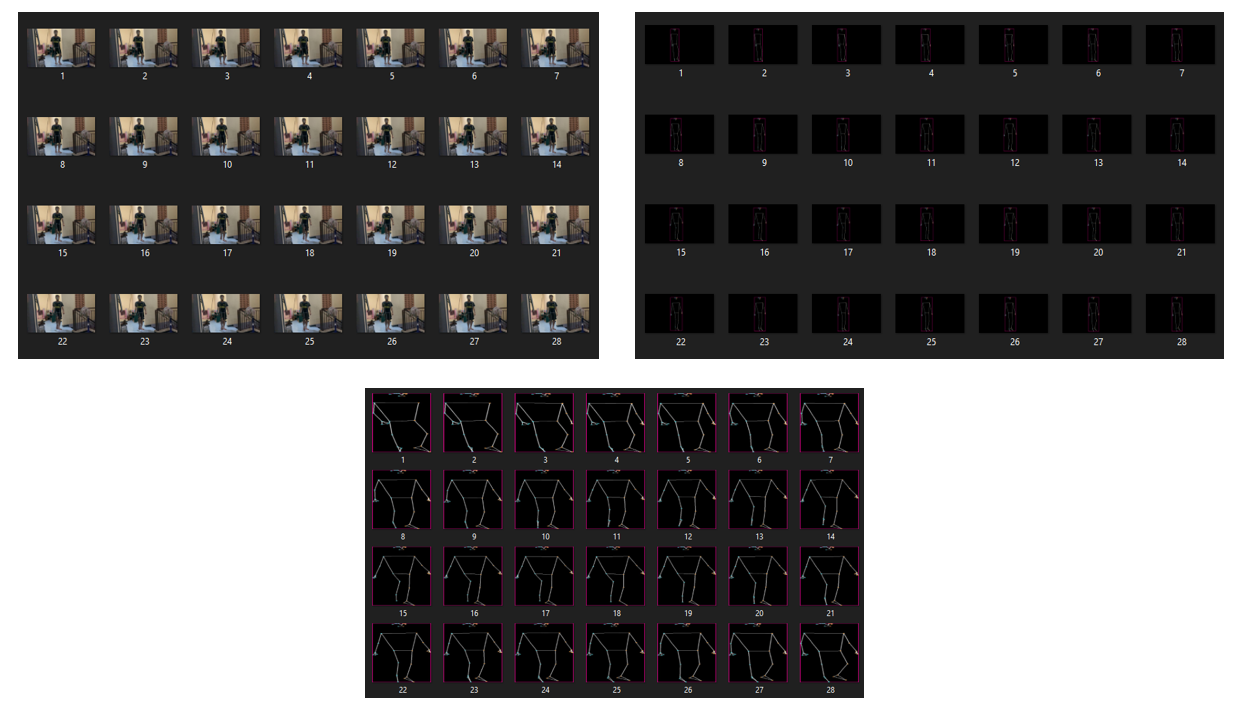
\includegraphics[scale=0.48]{gambar/dataset.png}
    % Keterangan gambar yang diinputkan
    \caption{Data gambar percobaan}
    % Label referensi dari gambar yang diinputkan
    \label{fig:Dataset}
\end{figure}

% Contoh input gambar dengan format *.jpg
\begin{figure} [ht] \centering
    % Nama dari file gambar yang diinputkan
    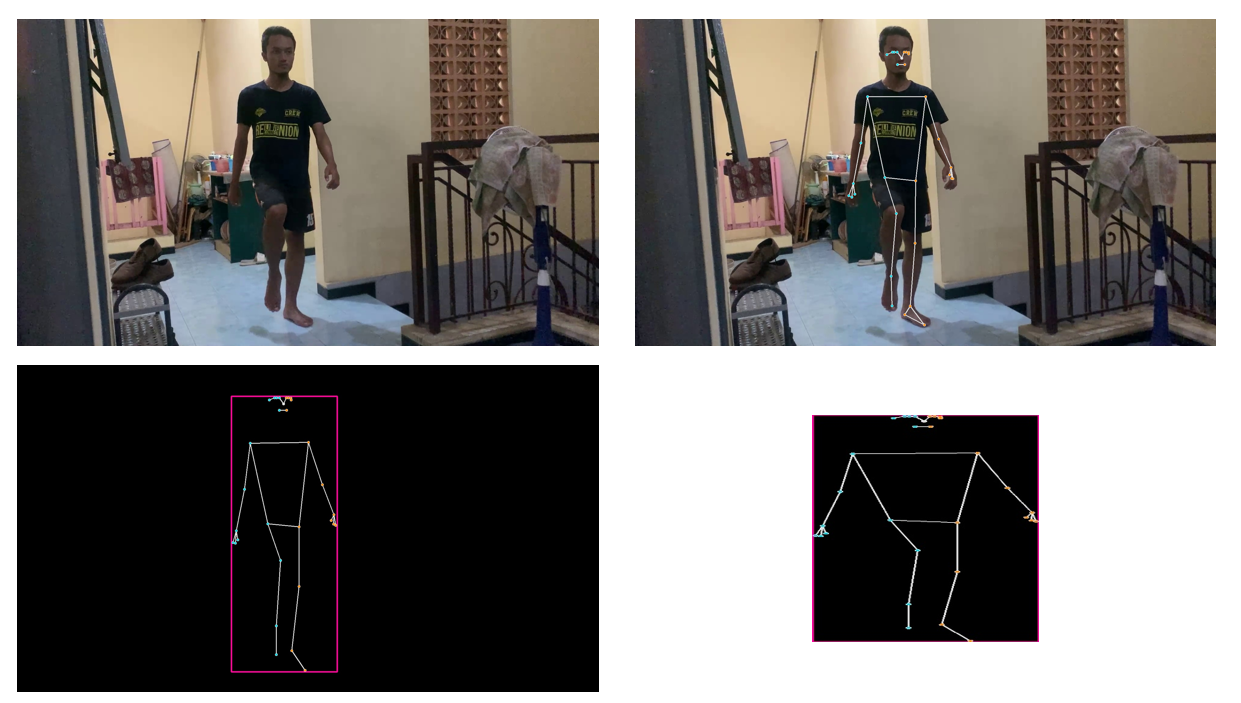
\includegraphics[scale=0.48]{gambar/estimasi ekstrak.png}
    % Keterangan gambar yang diinputkan
    \caption{Percobaan estimasi pose dan ekstrak fitur}
    % Label referensi dari gambar yang diinputkan
    \label{fig:EstimasiEkstrak}
\end{figure}

  \cleardoublepage

  % Daftar pustaka
  \chapter*{DAFTAR PUSTAKA}
  \addcontentsline{toc}{chapter}{DAFTAR PUSTAKA}
  \renewcommand\refname{}
  \vspace{2ex}
  \renewcommand{\bibname}{}
  \begingroup
    \def\chapter*#1{}
    \printbibliography
  \endgroup


\end{document}
